
%!TEX encoding = UTF-8 Unicode
\documentclass{oblivoir}
\usepackage{mathtools} %gathered 환경
\usepackage{graphics}

\author{Taewon Kang (itschool@itsc.kr)}
\title{\TeX를 사용한 수식 표현}
\begin{document}
	\maketitle
		\begin{equation} 
			x = \frac{-b\pm \sqrt{b^2-4ac}}{2a} \label{1}
		\end{equation}
		\LaTeX에서 \verb|\frac{-b\pm \sqrt{b^2-4ac}}{2a}| 구문을 사용하여, 근의 공식 \ref{1}을 위와 같이 표현할 수 있다.
		
		\begin{equation}
			\begin{gathered}
				\alpha + \beta = -\frac{b}{a} \label{2}
			\end{gathered}
		\end{equation}	
			
		\begin{equation}
			\begin{gathered}
				\alpha \beta = \frac{c}{a} \label{3}
			\end{gathered}
		\end{equation}
		
		\begin{align} %독립적인 수식 환경, equation 내 사용 불가
			1 + 2 + 3 + \cdots + n &= \sum_{k=1}^{n}k \nonumber \\
			&= \frac{1}{2}\sum_{k=1}^{n}(k+(n+1-k)) \nonumber \\
			&= \frac{1}{2}\sum_{k=1}^{n}(n+1) \nonumber \\
			&= \frac{n(n+1)}{2}
		\end{align}
		\TeX에서 수열의 합을 나타내는 식은 위와 같이 쓸 수 있다. $\sum_{k=1}^{n}k$ 기호는 \verb|\frac{\sum_{k=1}^{n}k}| 구문으로 쓸 수 있다. 등호를 기준으로 식을 정렬하고 싶은 경우 \verb|&=| 을 사용한다. 
\footnote{usepackage(mathtools) 을 전처리부에 반드시 삽입해 주어야 한다.}

\vspace{10pt} 

our school Assignments: \emph{The Precise Definition of a Limit}
	\begin{enumerate}
		\item Prove the limit statement. (Use $\epsilon$-$\delta$ Definition for proving statements.)\\
 		\begin{equation}
 			\lim_{x \to 3}{2x-1} = 5 \nonumber
 		\end{equation}
		
		\item Prove the limit statement. (Use $\epsilon$-$\delta$ Definition for proving statements.)\\
 		\begin{equation}
 			\lim_{x \to 2}{\frac{x^2-4}{x-2}} = 4 \nonumber
 		\end{equation}

		\item Prove the limit statement. (Use $\epsilon$-$\delta$ Definition for proving statements.)\\
 		\begin{equation}
 			\lim_{x \to 3}{x^2} = 9 \nonumber
 		\end{equation}
		
		\item Prove the limit statement. (Use $\epsilon$-$\delta$ Definition for proving statements.)\\
 		\begin{equation}
 			\lim_{x \to a}{\sin x} = \sin a \nonumber
 		\end{equation}
		
		이 문제의 해답은 아래와 같다. $|sin(x)| < |x|$는 그림으로 파악할 것. \\
		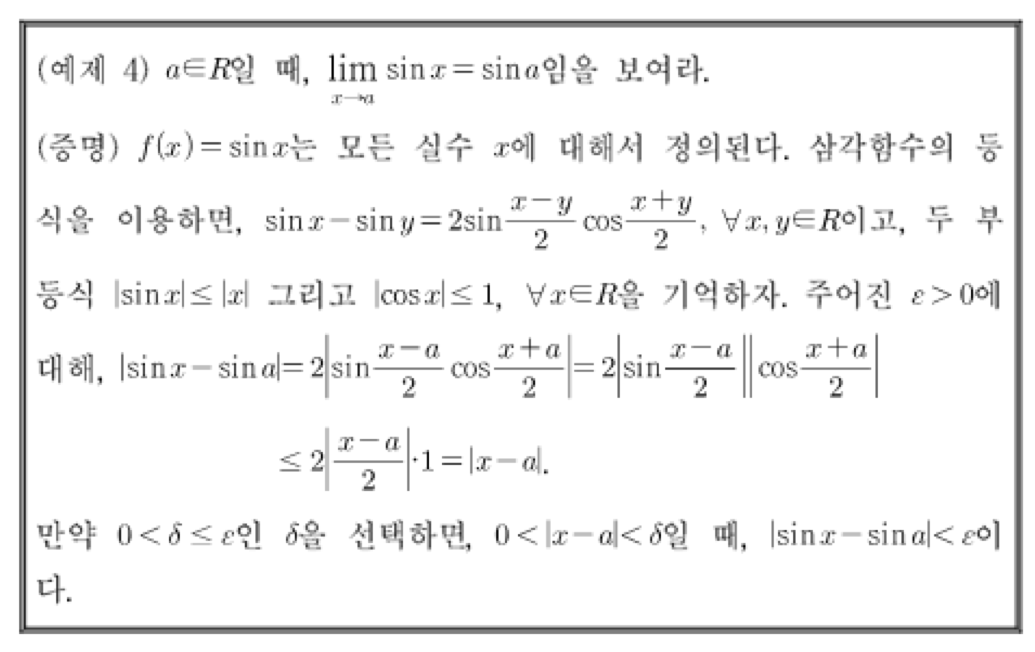
\includegraphics[width=1.0\textwidth]{solution3.png}
		
		\item Prove the limit statements. (Use $\epsilon$-$\delta$ Definition for proving statements.)\\
 		\begin{equation}
 			\lim_{x \to a}{\sqrt{x}} = \sqrt{a} \nonumber (when a < 0)
 		\end{equation}
		
		\item Prove the limit statement. (Use $\epsilon$-$\delta$ Definition for proving statements.)\\
 		\begin{equation}
 			\lim_{x \to -1}{\frac{x}{2x+1}} = 1 \nonumber
 		\end{equation}
		
	\end{enumerate}
\end{document}